% \documentclass[12pt]{article}
\documentclass[12pt]{diazessay}
% \usepackage{bashful}
\usepackage{hyperref}
% \usepackage{verbatim}
% \usepackage{graphics}
% \usepackage{algpseudocode}
% \usepackage{algorithm}


%----------------------------------------------------------------------------------------
%	TITLE SECTION
%----------------------------------------------------------------------------------------

\title{\texttt{\huge{Image Processing Using MPI\\\vspace{-3mm}} \vspace{-0.35cm} {\large CSCI 79300 Independent Study Report}\\\normalsize\url{https://github.com/chuanyao17/Image-Processing-Using-MPI}}} % Title and subtitle

\author{\texttt{Chuanyao Lin}\vspace*{-0.25em}} % Author and institution

\date{\texttt{\today}} % Date, use \date{} for no date

%----------------------------------------------------------------------------------------

\begin{document}

\maketitle
\section*{Abstract}
Image Processing Using MPI Project presents the technique of parallel computing while editing an image. The project includes different image functions such as image zooming, image rotation, image brightness and contrast adjustment, image blurring, and image gray-scale converting. First, an input image file will be converted to a matrix. Since the listed image processing functions contain a lot of matrix computations, they are highly parallelizable. After each scattered matrix is computed in parallel during different functions, they can be combined and converted into an image file again with the edited appearance. The running time is improved by a factor of number of processes used.
\section*{Introduction}
Message Passing Interface (MPI) which is a library to achieve a message-passing model to the sequential language like C, C++ is mainly used to parallelize the matrix computations. In this project,
the main concept to run a program in parallell is by adopting a message-passing model. The advantage of using a message-passing model is that it can be used in a distributed environment rather than processes on a single processor or the communicating processes reside on the same machine sharing a common address space. The goal of this project is to improve the computational time by running the image processing functions in parallel.
 
\section*{Methodology}
The following algorithm explains the process to run the image processing functions in parallel through MPI.
\begin{enumerate}
    \item Get the size and the rank of processes.
    \item Root process reads the input image.
    \item Root process broadcasts the properties of the input image to other processes.
    \item Scatter the input image among each process.
    \item Each process gets the edited image in parallel by different image processing functions based on the scattered input image.
    \item Gather all the edited images to the root process to become a whole edited image.
\end{enumerate}
In general, the sequential image processing function will go through each pixel of the input image independently and modified it with different algorithms. The main idea to run the image processing function in parallel is to scatter the input image among each process, so that each process will do the same algorithm to get different part of the edited image in parallel. After all the processes have done the computations, we can simply gather all the edited images to be a whole edited image. Therefore, the "shape" of the scattered input image will be a problem to be solved in different image processing functions.

According to the image processing functions mentioned above, the ways to scatter the input image can be divided into the following three categories.
\begin{enumerate}
    \item Row-wise block striped decomposition
    \item Row-wise block striped decomposition with overlapping border
    \item Column-wise block striped decomposition
\end{enumerate}

For the \textbf{row-wise block striped decomposition}, since the input image can be decomposed as the adjacency matrix, it can also be scattered by sets of adjacency rows to each process, as shown in Figure \ref{row_wise}.
\begin{figure}[h]
    \centering
	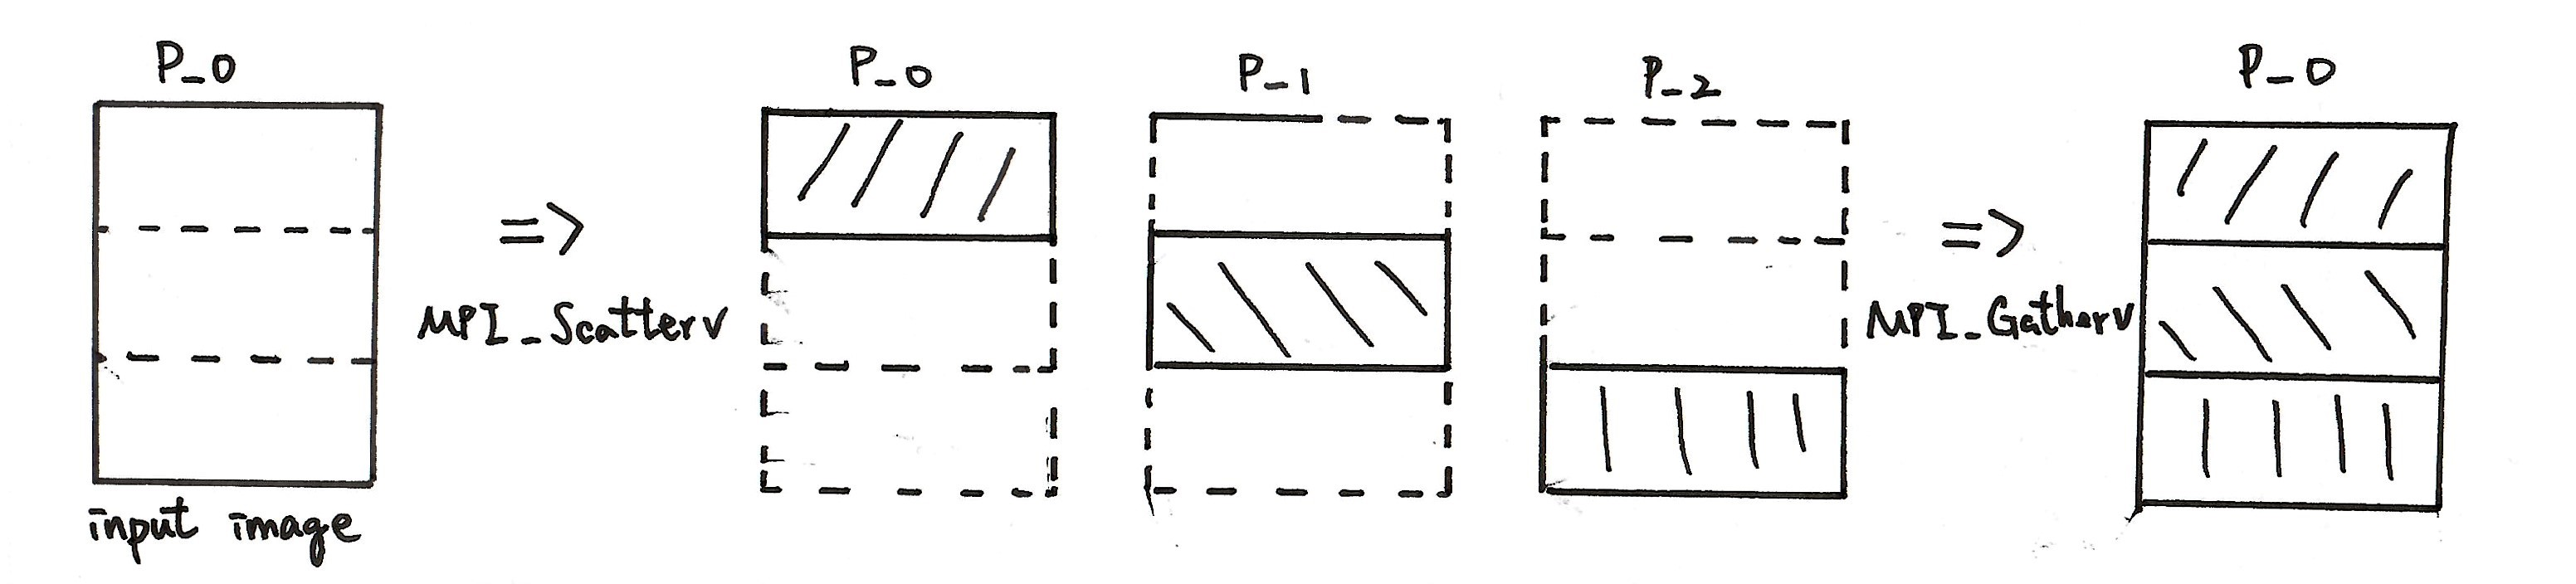
\includegraphics[scale=0.6, clip]{pics/row_wise.jpg}
	\caption {Row-wise block striped decomposition}
	\label{row_wise}
\end{figure}
\newline
In the project, the functions \textit{image brightness and contrast adjustment}, and \textit{image gray-scale converting} will be using this method to receive different parts of input image. The main idea of these functions to calculate the output image is based on the each pixel of the source image as follows. $$dst(i,j)= g(src(i,j))$$ (i,j) represents the 2D coordinates of the image. dst(i,j) and src(i, j) represent the pixel's color of the image at (i,j). g(x) represents the different image processing functions. For \textit{image brightness and contrast adjustment}, the function g(x) is considered as $$g(src(i,j))=alpha *src(i,j) + beta$$alpha represents the ratio of contrast, and beta is the number of increasing brightness\cite{Opencv}. For \textit{image gray-scale converting}, the function g(x) is considered as $$g(src(i,j))= src_{red}(i,j)*0.299 + src_{green}(i,j)*0.587 + src_{blue}(i,j)*0.114$$  \cite{Matlab}.That is, based on the size of the scattered image each process received, each process will produce the modified output image with the same size as the scattered image.  
However, compare to the previous two functions, there is a slight difference of the function \textit{image zooming}. Since the size of the output image will be changed by the zooming ratio, we'll use the bilinear interpolation to get the color of the corresponding coordinates from the source image. 

For the \textbf{row-wise block striped decomposition with overlap}, it's used in the function \textit{image blurring}. Since the method to get blurring image is to apply matrix convolution with the specific kernel matrix, we need to add additional borders of the source image to do the matrix convolution of each pixel before scattering it. For example, if we applied a 3x3 kernel matrix, we'll need to add 2 more rows and columns around the input image first. The method used to create border here is by copy the pixel as follows. $$gfedcb|abcdefgh|gfedcba$$ Compare to the previous scatter method, each scattered image will need the additional rows and columns to form the border. That is, there are overlapping parts between each scattered image. See Figure \ref{row_wise_overlap}.
\begin{figure}[h]
    \centering
	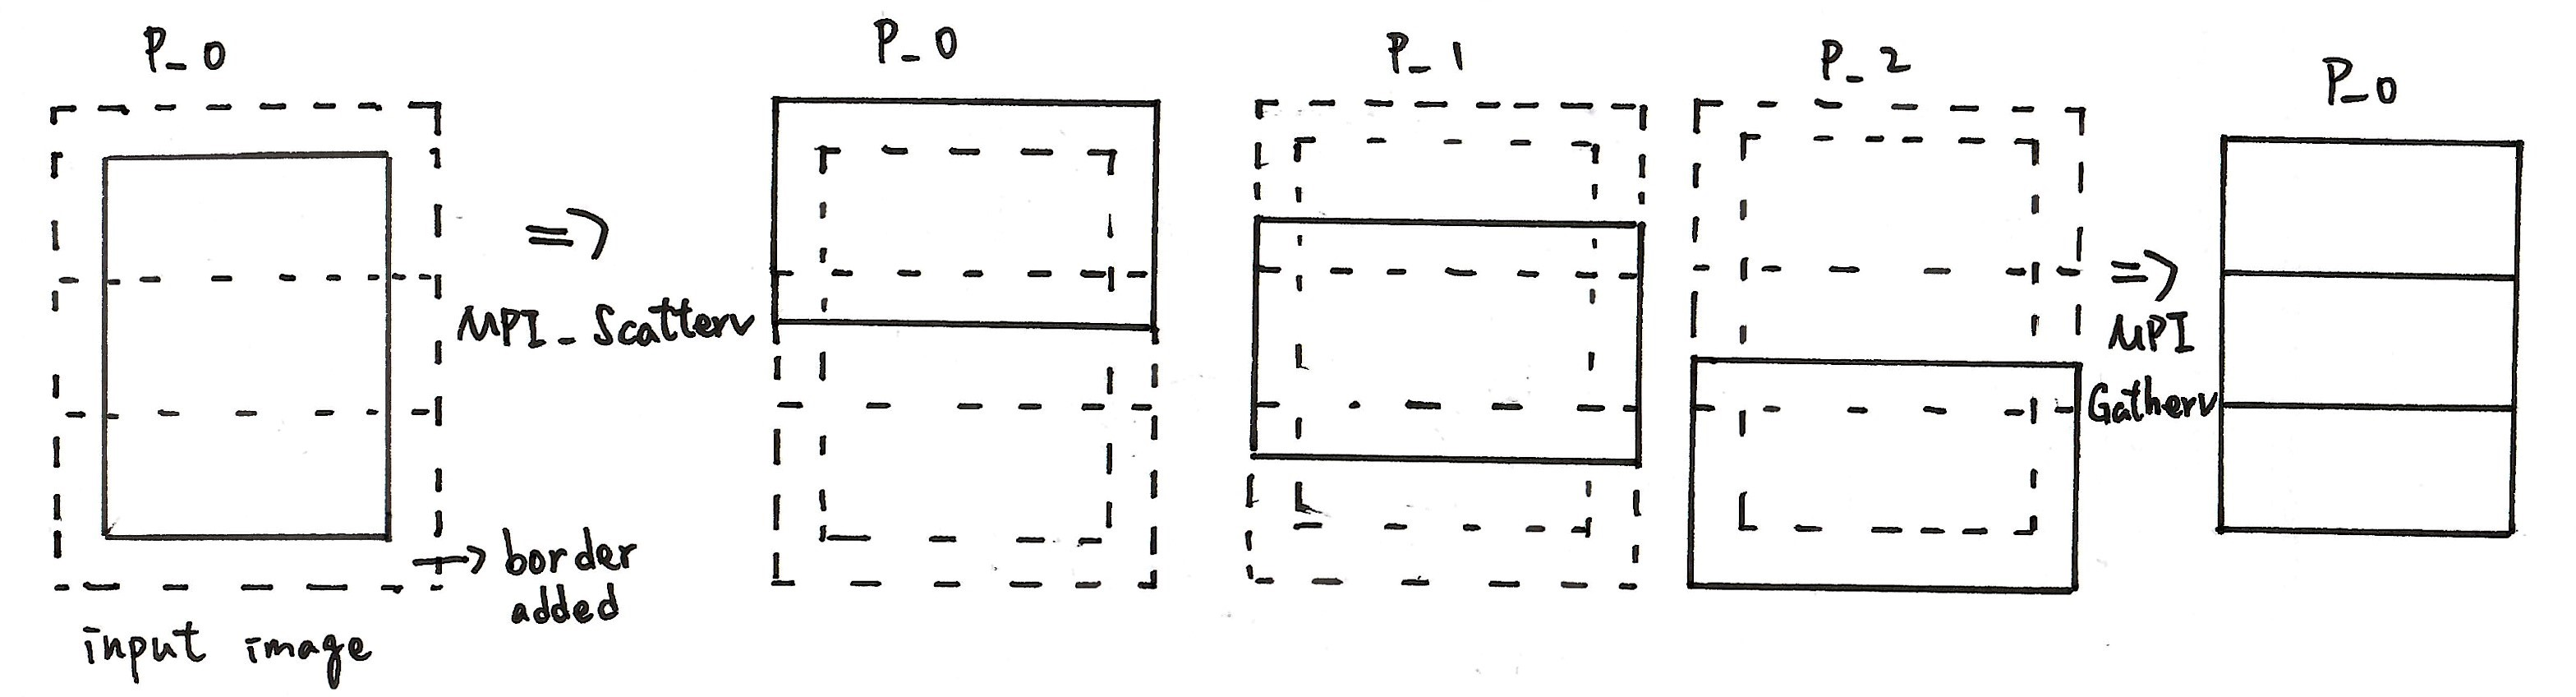
\includegraphics[scale=0.6, clip]{pics/row_wise_overlap.jpg}
	\caption {Row-wise block striped decomposition with overlapping border}
	\label{row_wise_overlap}
\end{figure}
\newline
Root process contains the added upper side border of the input image, and the additional rows of the input image at the bottom of the scattered image like $P\_0$ in Figure \ref{row_wise_overlap}. The last process contains the added lower side border of the input image and the additional rows of the input image at the top of the scattered image like $P\_2$ in Figure \ref{row_wise_overlap}. Processes between the root and last process will contain additional rows of the scattered image at the both top and bottom side like $P\_1$ in Figure \ref{row_wise_overlap}.

For the \textbf{Column-wise block striped decomposition}, it's used in the function \textit{image rotation}. Unlike scattering the input image in row-wise, in order to do the coordinate transformation of the rotation, the input image will be scattered in column-wise as follows. See Figure\ref{col_wise}
\newline
\begin{figure}[h]
    \centering
	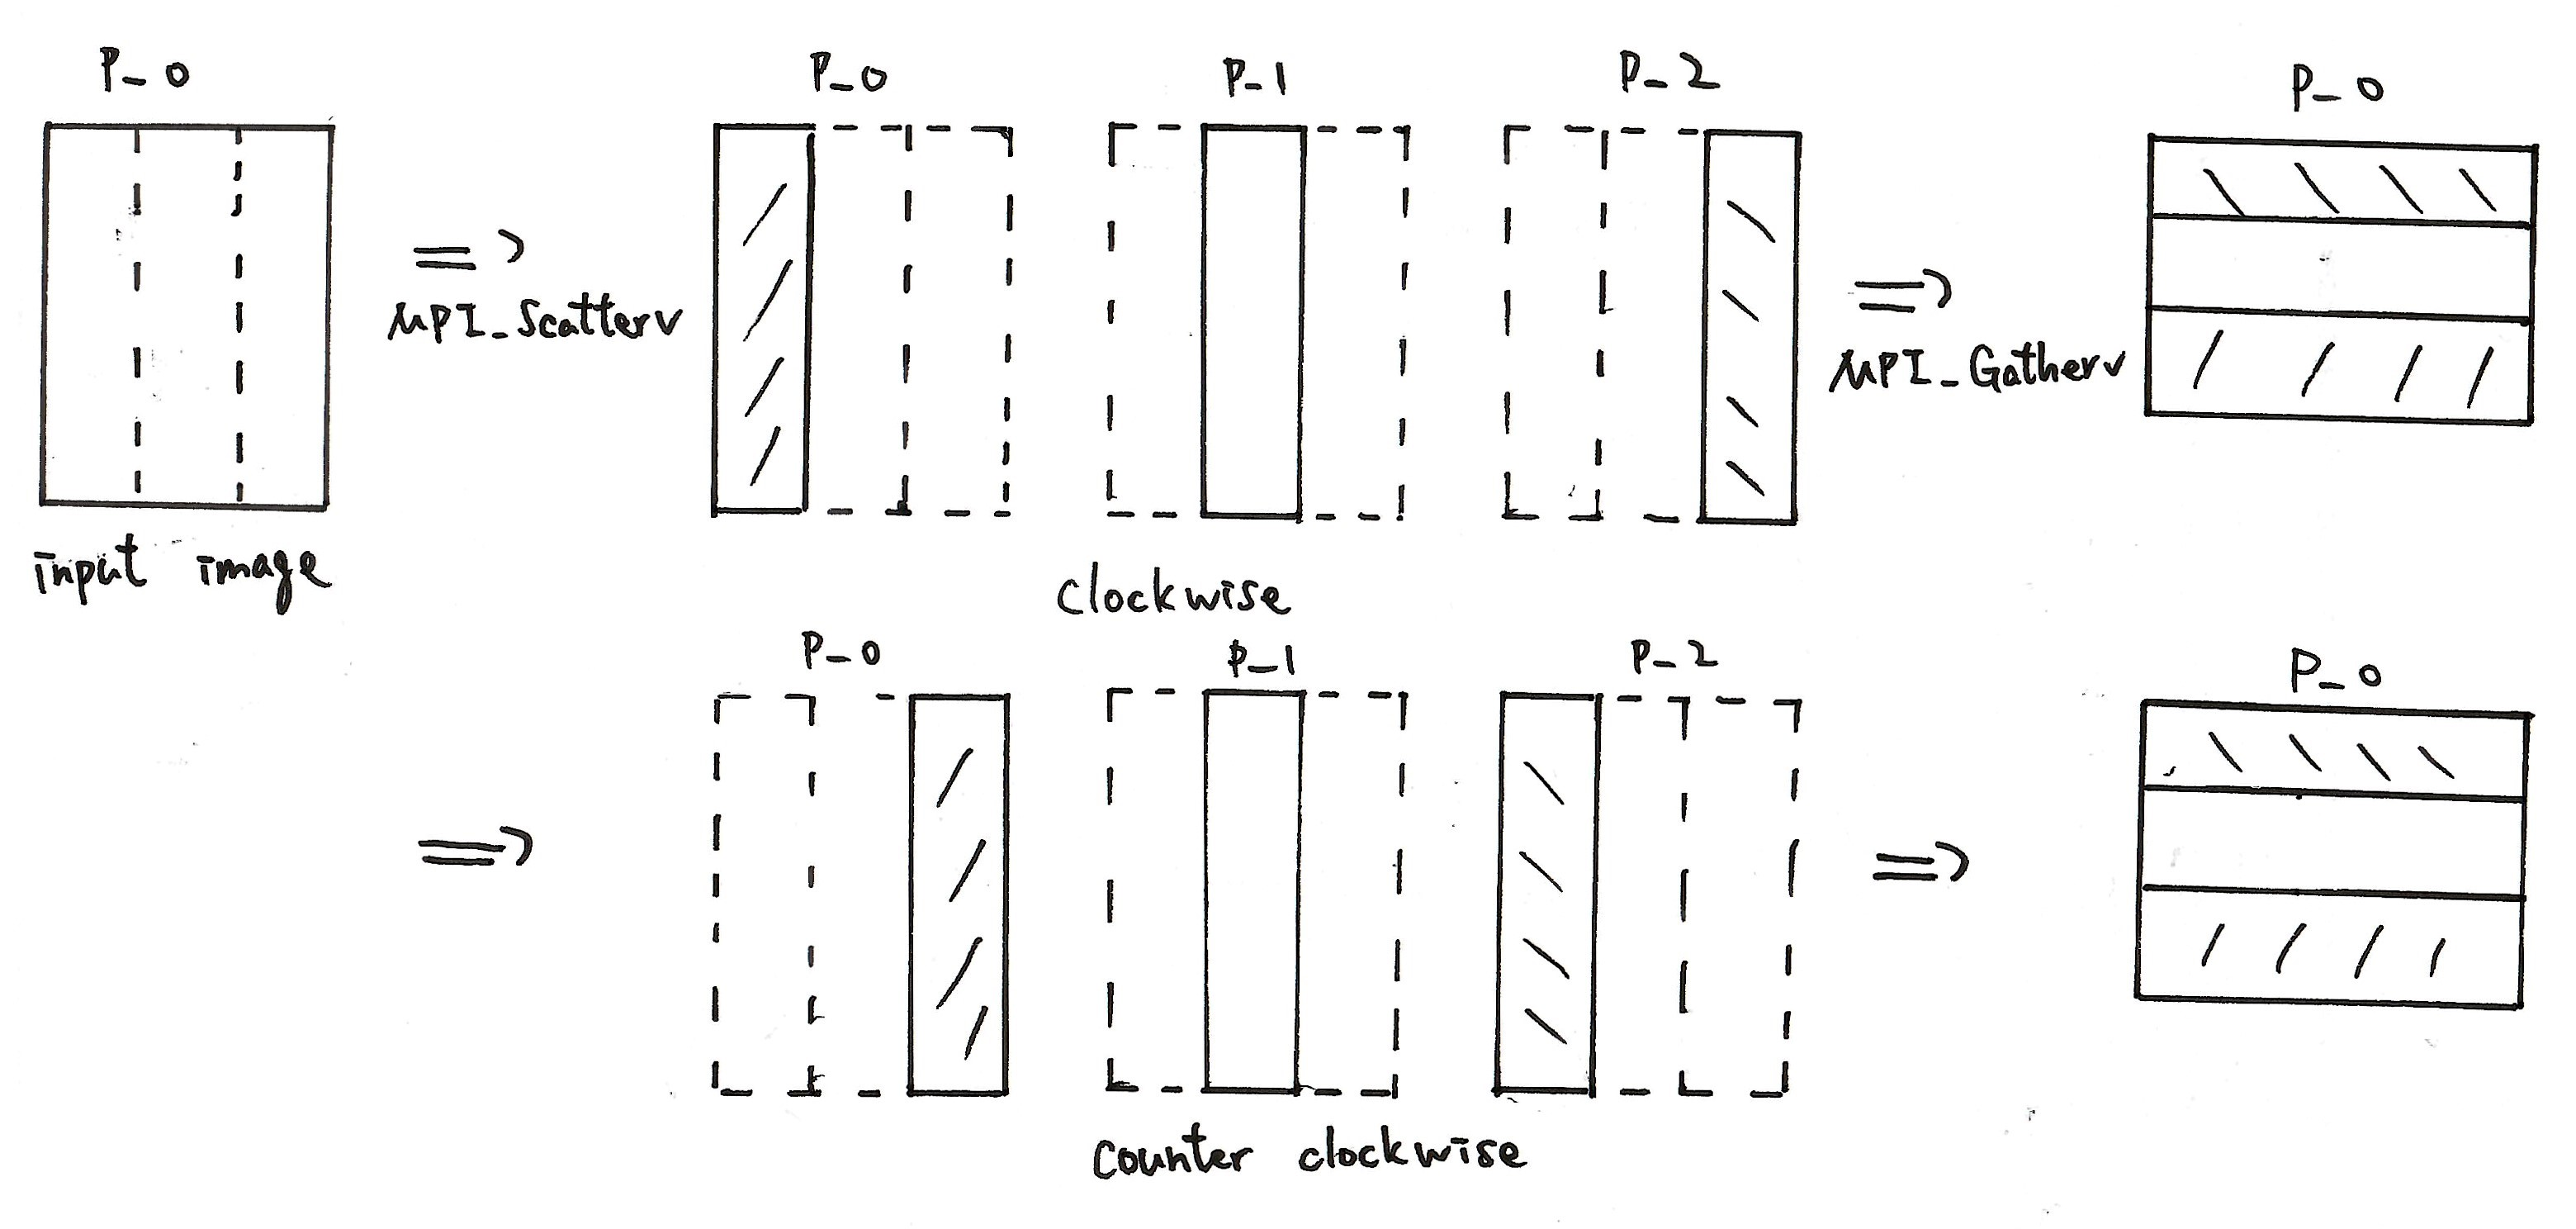
\includegraphics[scale=0.6, clip]{pics/col_wise.jpg}
	\caption {Column-wise block striped decomposition}
	\label{col_wise}
\end{figure}
\newline
Once the process received the scattered input image, the roatated output image can be calculated as follows. $$dst(i,j)=src(r*j,-r*i)$$ r will be -1 if the image rotates in clockwise direction, and 1 if in counter-clockwise direction. One more difference between above two rotation directions is that the input image needs to be scattered in opposite index, since MPI\_Gatherv always gathers the data from the root process.

Lastly, there is one more problem (coordinate transformation) which needs to be dealt with during running the image processing functions in parallel. First, every scattered image's coordinate always starts from (0,0). Second, unlike the Cartesian coordinate system, the image's index(row or y-axis) increases from top to bottom. Third, the scattered image needs to be aligned with the input image. Therefore, we need extra effort like considering the index offset in order to get the right corresponding coordinates in different functions.   
\clearpage
\section*{Results}

Below are the results of different image processing functions running in parallel with the same environment. \footnote{Image brightness and contrast adjustment has the similar result with the image gray-scale since the only difference is the way to change the color of each pixel.}


\begin{table}[h]
\centering
\begin{tabular}{|l|l|lll}
\cline{1-2}
\textbf{Number of Processes} & \textbf{\begin{tabular}[c]{@{}l@{}}Time taken to run the image gray-scale \\ (seconds)\end{tabular}} &  &  &  \\ \cline{1-2}
1 & 0.679385 &  &  &  \\ \cline{1-2}
2 & 0.346514 &  &  &  \\ \cline{1-2}
3 & 0.280369 &  &  &  \\ \cline{1-2}
4 & 0.249300 &  &  &  \\ \cline{1-2}
5 & 0.266033 &  &  &  \\ \cline{1-2}
6 & 0.246622 &  &  &  \\ \cline{1-2}
\end{tabular}
\caption{Image gray-scale using the size $4000\times 4000$ color image}
\end{table}

\begin{table}[h]
\centering
\begin{tabular}{|l|l|lll}
\cline{1-2}
\textbf{Number of Processes} & \textbf{\begin{tabular}[c]{@{}l@{}}Time taken to run the image blurring  \\ (seconds)\end{tabular}} &  &  &  \\ \cline{1-2}
1 & 22.078334 &  &  &  \\ \cline{1-2}
2 & 11.830913 &  &  &  \\ \cline{1-2}
3 & 11.756907 &  &  &  \\ \cline{1-2}
4 & 12.114337 &  &  &  \\ \cline{1-2}
5 & 12.267256 &  &  &  \\ \cline{1-2}
6 & 11.542304 &  &  &  \\ \cline{1-2}
\end{tabular}
\caption{Image blurring(average blur) using the size $4000\times 4000$ color image and $9\times 9$ kernel matrix}
\end{table}

\clearpage

\begin{table}[h]
\centering
\begin{tabular}{|l|l|lll}
\cline{1-2}
\textbf{Number of Processes} & \textbf{\begin{tabular}[c]{@{}l@{}}Time taken to run the image rotation \\ (seconds)\end{tabular}} &  &  &  \\ \cline{1-2}
1 & 0.202791 &  &  &  \\ \cline{1-2}
2 & 0.155099 &  &  &  \\ \cline{1-2}
3 & 0.136452 &  &  &  \\ \cline{1-2}
4 & 0.137103 &  &  &  \\ \cline{1-2}
5 & 0.114158 &  &  &  \\ \cline{1-2}
6 & 0.122135 &  &  &  \\ \cline{1-2}
\end{tabular}
\caption{Image rotation in clockwise using the size $4000\times 4000$ color image }
\end{table}

\begin{table}[h]
\centering
\begin{tabular}{|l|l|lll}
\cline{1-2}
\textbf{Number of Processes} & \textbf{\begin{tabular}[c]{@{}l@{}}Time taken to run the image zooming\\ (seconds)\end{tabular}} &  &  &  \\ \cline{1-2}
1 & 3.676640 &  &  &  \\ \cline{1-2}
2 & 2.296864 &  &  &  \\ \cline{1-2}
3 & 2.093839 &  &  &  \\ \cline{1-2}
4 & 1.508312 &  &  &  \\ \cline{1-2}
5 & 1.719045 &  &  &  \\ \cline{1-2}
6 & 2.076345 &  &  &  \\ \cline{1-2}
\end{tabular}
\caption{Image zooming using the size $282\times 147$ color image and zooming it to the size $3948\times 3969$}
\end{table}
From the above tables, the results show that as the number of processes increases, the time reduces by a factor of number of processes. However, there is a limitation of improvement for increasing the number of processes. We'll discuss the reason in the next section.
\clearpage
\section*{Performance Analysis}

In this section, we're talking about the time complexity and scalability of running the image processing functions in parallel. For an $m\times n$ size of input image, since every image processing function in sequential in this project has time complexity $\Theta(mn)$, so we'll only discuss the difference between the \textbf{Row-wise block striped decomposition} and \textbf{Column-wise block striped decomposition}.\footnote{Row-wise block striped decomposition with overlapping border has the same time complexity as Row-wise block striped decomposition.} Although the time complexity of the image blurring function is actually $\Theta(m\times n \times o \times p)$ where $o \times p$ is the size of the kernel matrix, we assume the kernel size is fixed. Moreover, to simplify the analysis, we'll assume the shape of the input image is square, so the time complexity in sequential will become $\Theta(n^2)$.
Before we start to determine the time complexity of the portion of the algorithms, we won't include the time spent performing I/O, since both sequential and parallel algorithm have to read the input image. Also, we won't include the overhead of distributing the input image to each process, since the time complexity is rather smaller than the time complexity of the image processing function itself. 

For the \textbf{Row-wise block striped decomposition}, each task has at most $[n/p]$ rows and n columns of the input image. Therefore, the time complexity of the computational part of each task of the parallel algorithm is $\Theta(n^2/p)$.\cite{ch7} The communication time complexity is the result(output) image replicated in every task by MPI\_Gatherv. If MPI uses the hypercube based approach, the time complexity will be $\Theta(\log p + n)$. In short, the total time complexity will be $\Theta((n^2/p)+\log p + n)$. However, if p is much smaller than n, the total time complexity will be $\Theta((n^2/p))$. For the scalability, we can check the isoefficiency relation of the algorithm. Since the time complexity of the sequential algorithm is $\Theta(n^2)$, $T(n,1)=n^2$. The parallel overhead $T_0(n,p)$ only takes place after each task finishing the image processing and assembling to a whole edited image by using the MPI\_Gatherv. Assuming the size of input image is much larger than the number of processes, the time complexity is $n(p-1)/\beta p$, which is $\Theta(n)$. $\beta$ denotes the transfer time of the channel's bandwidth. Therefore $T_0(n,p) = np$, the isoefficiency relation is as follows, $$T(n,1)\geq C \cdot T_0(n,p) \rightarrow n^2\geq Cnp \rightarrow n\geq Cp$$ Since the memory storage is $\Theta(n^2)$, the memory utilization function is $M(n)=n^2$. According to the the scalability function $M(f(p))/p$, $$M(Cp)/p=(Cp)^2/p=C^2p$$ In conclusion, in order to maintain the efficiency as the number of processes is increased, the memory per process needs to grow as the number of processes increasing. In other words, it's not scalable of this algorithm for large number of processes.

For the \textbf{Column-wise block striped decomposition}, the only difference from the previous one is that each task has at most $[n/p]$ columns and n rows of the input image. However, the rest of the analyzing will be same. In fact, some of the image processing function in the project, MPI\_Bcast and MPI\_Allgather have been used to calculate the communication arrays for using MPI\_Gatherv and MPI\_Scatterv. However, they're ignored in the above analyzing since the computational time is also rather smaller than the time of image processing function itself.
 



\clearpage
\begin{thebibliography}{00}
\bibitem{Quinn}M.J. Quinn. Parallel Programming in C with MPI and OpenMP. McGraw-Hill Higher Education. McGraw-Hill Higher Education, 2004.
\bibitem{Opencv}Bradski, G. (2000). The OpenCV Library. Dr. Dobb's Journal of Software Tools.
\bibitem{Matlab}MATLAB. (2010). version 7.10.0 (R2010a). Natick, Massachusetts: The MathWorks Inc.
\bibitem{ch7}Weiss, S. (n.d.). CSci 493.65 Parallel Computing Chapter 7 Matrix-Vector Multiplication. Retrieved May 20, 2022, from \url{http://www.compsci.hunter.cuny.edu/~sweiss/course_materials/csci493.65/lecture_notes/chapter07.pdf }

\end{thebibliography}

\end{document}
